\documentclass[twocolumn]{article}

% Packages
\usepackage[utf8]{inputenc}
\usepackage{amsmath, amssymb}
\usepackage{xcolor, graphicx}
\usepackage{float, caption}
\usepackage{geometry}
\usepackage{array, enumitem}
\usepackage{url}
\usepackage{cuted} % For single-column title in two-column layout
\geometry{margin=1in}
\pagestyle{empty}

\begin{document}

% One-column title section using 'strip'
\begin{strip}
\vspace*{10em}  % Adjust vertical spacing as needed
\begin{minipage}{0.45\textwidth}
    \includegraphics[width=\textwidth]{WhatsApp Image 2025-07-08 at 3.59.18 PM.jpeg}
\end{minipage}\hfill
\begin{minipage}{0.45\textwidth}
    \textbf{Name: Madhu Latha G } \\
    \textbf{ID: cometfwc029} \\
    \textbf{Date: 7th June 2025} \\
\end{minipage}
\vspace{-7em}
\begin{center}
    {\LARGE \textbf{\textcolor{cyan}{GATE Question Paper 2010, EE Question Number 52}}}
\end{center}
\end{strip}

% Two-column content starts here

\section*{\textcolor{blue}{Question 12 Analysis}}
\textcolor{blue}{\textbf{Question:}}

\begin{figure}[H]
    \centering
    \includegraphics[width=0.55\textwidth]{52.png}
\end{figure}

\section*{\textcolor{blue}{Karnaugh Map Simplification Problem}}
\textbf{Given:} The following Karnaugh map represents a function $F$:

\section*{\textcolor{blue}{Step-by-Step Solution}}
\begin{enumerate}
    \item \textbf{Identify variables:}
    \begin{itemize}
        \item Variables: $X$, $Y$, $Z$
        \item Columns in Gray code: 00, 01, 11, 10
    \end{itemize}

    \item \textbf{Extract minterms:}
    \begin{itemize}
        \item 1s at: $(0,00), (0,01), (0,11), (1,01)$
        \item Minterms:
        \begin{align*}
            & (0,00) \rightarrow \overline{X}\,\overline{Y}\,\overline{Z} \\
            & (0,01) \rightarrow \overline{X}\,\overline{Y}\,Z \\
            & (0,11) \rightarrow \overline{X}\,Y\,Z \\
            & (1,01) \rightarrow X\,\overline{Y}\,Z
        \end{align*}
    \end{itemize}

    \item \textbf{Group minterms:}
    \begin{itemize}
        \item Group 1: $\overline{X}\,\overline{Y}$
        \item Group 2: $\overline{X}\,Y\,Z + X\,\overline{Y}\,Z = YZ$
    \end{itemize}

    \item \textbf{Final Expression:}
    \[
        F = \overline{X}\,\overline{Y} + YZ
    \]
\end{enumerate}
% ---------------------- Pico W -----------------------
\vspace{-2.5em}
\section*{\textcolor{blue}{Implementation using Pico W}}

\section*{\textcolor{blue}{Abstract}}
This part replicates the same logic on Raspberry Pi Pico W using MicroPython via Thonny IDE.

\section*{\textcolor{blue}{Hardware Requirements}}
\begin{table}[H]
\renewcommand{\arraystretch}{1.3}
\begin{tabular}{|c|l|}
\hline
\textbf{S.No} & \textbf{Component} \\ \hline
1 & Raspberry Pi Pico W \\
2 & Breadboard \\
3 & Push Buttons (X, Y, Z) \\
4 & LED \\
5 & Resistors: 220$\Omega$, 10k$\Omega$ \\
6 & Jumper Wires \\
7 & Micro USB Cable \\
\hline
\end{tabular}
\caption*{\textbf{Table 1: Hardware Components}}
\end{table}

\section*{\textcolor{blue}{Pin Connections}}
\begin{table}[H]
\renewcommand{\arraystretch}{1.3}
\begin{tabular}{|c|c|}
\hline
\textbf{Component} & \textbf{Pico W Pin} \\ \hline
X & GP14 \\
Y & GP15 \\
Z & GP16 \\
F (LED) & GP13 \\
GND & GND \\
VCC & 3.3V \\
\hline
\end{tabular}
\caption*{\textbf{Table 2: GPIO Pin Config}}
\end{table}

\section*{\textcolor{blue}{Upload Steps}}
\begin{enumerate}[label=\arabic*.]
    \item Connect Pico W while holding BOOTSEL
    \item Copy .uf2 firmware to RPI-RP2
    \item Open Thonny IDE and set interpreter to Pico
    \item Write and run MicroPython code
    \item Connect hardware circuit and test
\end{enumerate}

\section*{\textcolor{blue}{Observations}}
\begin{table}[H]
\renewcommand{\arraystretch}{1.3}
\begin{tabular}{|c|c|c|c|}
\hline
X & Y & Z & F (LED) \\ \hline
0 & 0 & 0 & 1 \\
0 & 0 & 1 & 1 \\
0 & 1 & 1 & 1 \\
1 & 0 & 1 & 1 \\
1 & 1 & 0 & 0 \\
1 & 1 & 1 & 1 \\
\hline
\end{tabular}
\caption*{\textbf{Table 4: Truth Table}}
\end{table}

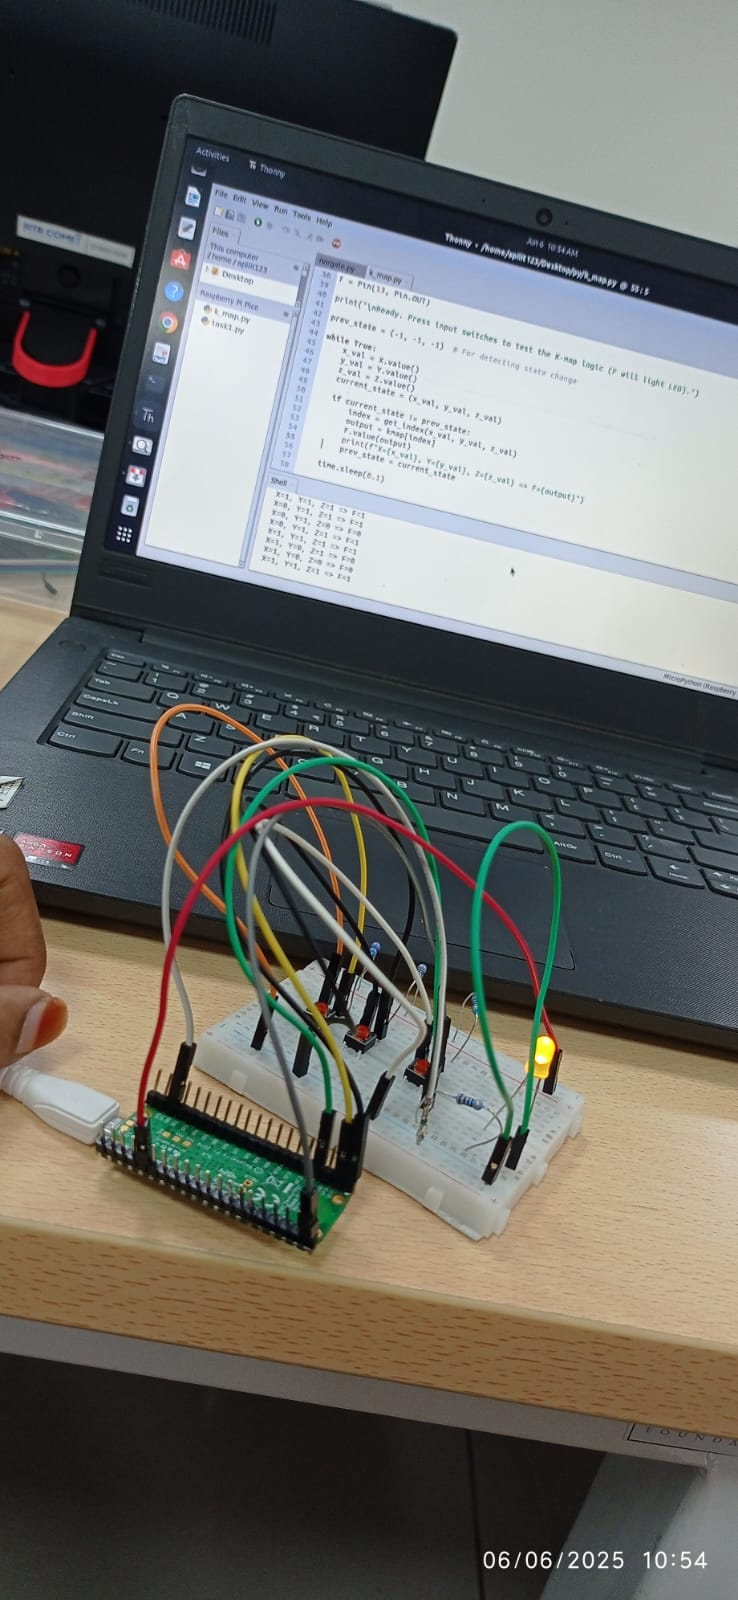
\includegraphics[width=0.45\textwidth]{hardware_task4.jpeg}
\url{https://github.com/madhuu34/Madhulathafwc/blob/main/Hardware/PLATFORM_IO/hardware_code.py}
\section*{\textcolor{blue}{Conclusion}}
The logic function was successfully tested on Pico W using MicroPython and validated with real input/output.

\end{document}
